\documentclass[conference]{IEEEtran}
\IEEEoverridecommandlockouts

\usepackage{cite}
\usepackage{amsmath,amssymb,amsfonts}
\usepackage{graphicx}
\usepackage{textcomp}
\usepackage{xcolor}
\usepackage{booktabs}
\usepackage{array}
\usepackage{tabularx}
\usepackage{hyperref}
\hypersetup{colorlinks=false}

\def\BibTeX{{\rm B\kern-.05em{\sc i\kern-.025em b}\kern-.08em
    T\kern-.1667em\lower.7ex\hbox{E}\kern-.125emX}}

\begin{document}

\title{Explainable Machine Learning Model for Early Prediction of Heart Disease}

\author{
\IEEEauthorblockN{[Author Name]}
\IEEEauthorblockA{
COM748 — MSc Research Project\\
[University Name]\\
[Email Address]}
}

\maketitle

% ─────────────────────────────────────────────────────────────────────────────
\begin{abstract}
Cardiovascular disease (CVD) remains the leading cause of death globally, yet early detection is hampered by cost and accessibility barriers. Machine learning offers predictive potential, but opaque models reduce clinical trust. This study presents an explainable ML framework for early heart disease prediction using the combined UCI heart disease dataset ($n{=}920$, four centres) under the CRISP-DM methodology. Five classifiers — Logistic Regression, Random Forest, XGBoost, SVM, and KNN — were evaluated across accuracy, precision, recall, F1, and AUC following median/mode imputation, IQR outlier capping, and SMOTE balancing applied strictly within stratified 5-fold cross-validation to prevent data leakage. Random Forest achieved the highest test AUC (0.916) with Precision\,=\,0.857 and Recall\,=\,0.882; SVM and XGBoost both achieved the highest recall (0.902), minimising missed diagnoses. Cross-validation AUC standard deviations remained below 0.041 across all models. SHAP analysis identified ST depression (\textit{oldpeak}), asymptomatic chest pain, and exercise-induced angina as the strongest global predictors, consistent with established cardiology literature. SHAP waterfall and LIME explanations for individual patients converged on the same clinical drivers, providing independent cross-validation of model reasoning. The framework adheres to the ACM Code of Ethics and BCS Code of Conduct, and is positioned as a decision support tool rather than an autonomous diagnostic system, demonstrating that interpretable ML can achieve high predictive accuracy with clinical explainability.
\end{abstract}

\begin{IEEEkeywords}
Heart disease prediction, Explainable AI, SHAP, LIME, SMOTE, Machine learning, CRISP-DM
\end{IEEEkeywords}

% ─────────────────────────────────────────────────────────────────────────────
\section{Introduction}

Cardiovascular disease (CVD) is the leading cause of death in the world, taking at least 17.9 million lives annually according to the World Health Organization \cite{who2025}. Early diagnosis is important because timely intervention can substantially reduce morbidity and mortality. Nevertheless, traditional diagnostic pathways — such as angiography and stress testing — are frequently inaccessible to disadvantaged groups due to cost and the scarcity of specialist clinicians. Machine learning (ML) offers a promising alternative, capable of analysing complex clinical data to identify individuals at risk \cite{hassija2023}.

However, high-performing models are often black boxes that do not reveal how decisions are made. This lack of transparency weakens clinical trust and inhibits adoption in settings where understanding the rationale behind a prediction is as important as the prediction itself \cite{banerjee2025}.

This study addresses that gap by developing an interpretable ML framework for early heart disease detection. The framework combines predictive modelling with explainability tools, enabling clinicians to interrogate and understand each prediction. The study uses the combined UCI heart disease dataset and follows the CRISP-DM methodology to ensure structured, reproducible, and transparent analysis \cite{desai2022}.

Five core objectives were defined: (1) preprocess the UCI data to handle missing values, encode categorical variables, normalise numeric features, and cap outliers using IQR; (2) address class imbalance using SMOTE applied exclusively within training folds to prevent data leakage; (3) benchmark five classifiers — Logistic Regression, Random Forest, XGBoost, SVM, and KNN — using accuracy, precision, recall, F1, and AUC under 5-fold stratified cross-validation; (4) apply SHAP and LIME for global and local explainability; and (5) ensure ethical deployment adhering to the ACM Code of Ethics and BCS Code of Conduct.

% ─────────────────────────────────────────────────────────────────────────────
\section{Literature Review}

\subsection{Machine Learning for Cardiovascular Disease Prediction}
A wide variety of classifiers have been tested on the UCI Cleveland heart disease dataset. Early studies relying on accuracy alone as the primary metric are methodologically flawed, as accuracy can mask poor minority-class performance in moderately imbalanced datasets \cite{ali2019}. Waqar et al.\ (2025) benchmarked five classifiers and found that ensemble methods (Random Forest and XGBoost) consistently outperformed individual learners, achieving AUC values above 0.90, with SHAP identifying chest pain type, maximum heart rate, and ST slope as dominant predictors \cite{lamir2025}. However, many studies lack structured preprocessing pipelines and fail to examine how class imbalance affects XAI importance scores \cite{uddin2026}.

\subsection{Class Imbalance and Over-sampling Techniques}
Class imbalance is a persistent challenge in medical classification. SMOTE \cite{fernandez2018} is the standard solution, generating synthetic minority samples to balance training data. A critical concern is that SMOTE must be applied \textit{inside} cross-validation folds to avoid data leakage \cite{yadav2020}. This study integrates SMOTE strictly within each CV fold, following best practice \cite{mujahid2024}.

\subsection{Explainable AI in Medicine}
SHAP (SHapley Additive exPlanations) provides theoretically grounded global feature importance based on cooperative game theory \cite{kim2025}. LIME \cite{ribeiro2016}, introduced by Ribeiro et al., provides local approximations by perturbing individual instances and fitting a sparse linear model. Few studies combine both techniques in a single CVD prediction system \cite{ahmed2024, admassu2023}. Ozdemir \cite{ozdemir2024} argues that dual-method XAI frameworks are essential for building clinical trust, as agreement between SHAP and LIME on the same patient strengthens confidence that the model responds to genuine clinical signals rather than data artefacts.

\subsection{Synthesis and Research Gap}
The literature demonstrates that ensemble classifiers achieve high accuracy in heart disease prediction, and that SHAP and LIME independently provide useful explanations. However, no study has combined: (1) a structured CRISP-DM pipeline, (2) SMOTE strictly inside CV folds, (3) five classifiers with full multi-metric evaluation, (4) both SHAP and LIME applied to the same patient for cross-validation of explanations, and (5) conceptual adversarial robustness evaluation. This study fills that gap.

% ─────────────────────────────────────────────────────────────────────────────
\section{Methodology}

\subsection{Research Design}
A quantitative, experimental, and comparative study design was adopted. Five classifiers were benchmarked using the same preprocessing and evaluation procedures \cite{sutanto2024}. The project lifecycle followed the six phases of CRISP-DM: business understanding, data understanding, data preparation, modelling, evaluation, and deployment considerations \cite{desai2022}.

\subsection{Data Source}
The dataset was sourced from the UCI Machine Learning Repository and comprises 920 patient records from four clinical centres: Cleveland ($n{=}304$), Hungary ($n{=}293$), VA Long Beach ($n{=}200$), and Switzerland ($n{=}123$). It contains 13 clinical features. The target variable was binarised: 0 = no disease ($n{=}411$, 44.7\%), 1 = disease present ($n{=}509$, 55.3\%).

\subsection{Data Preprocessing}
Missing values varied considerably across features: \textit{ca} (66.4\%), \textit{thal} (52.8\%), \textit{slope} (33.6\%), \textit{fbs} (9.8\%), \textit{oldpeak} (6.7\%), \textit{trestbps} (6.4\%), \textit{exang} and \textit{thalch} (6.0\% each), \textit{chol} (3.3\%), and \textit{restecg} (0.2\%). Categorical features were imputed using mode substitution; continuous features using median substitution. Physically impossible negative \textit{oldpeak} values (min $-2.6$) were clipped to zero prior to IQR capping, since ST depression cannot be negative by clinical definition. Outlier capping at $1.5 \times$ IQR was applied to \textit{age}, \textit{trestbps}, \textit{chol}, \textit{thalch}, and \textit{oldpeak}. The feature \textit{ca} was excluded from capping as it is a discrete integer count (0--3). Fig.~\ref{fig:outlier} shows before/after box plots confirming successful outlier removal.

\begin{figure}[htbp]
\centerline{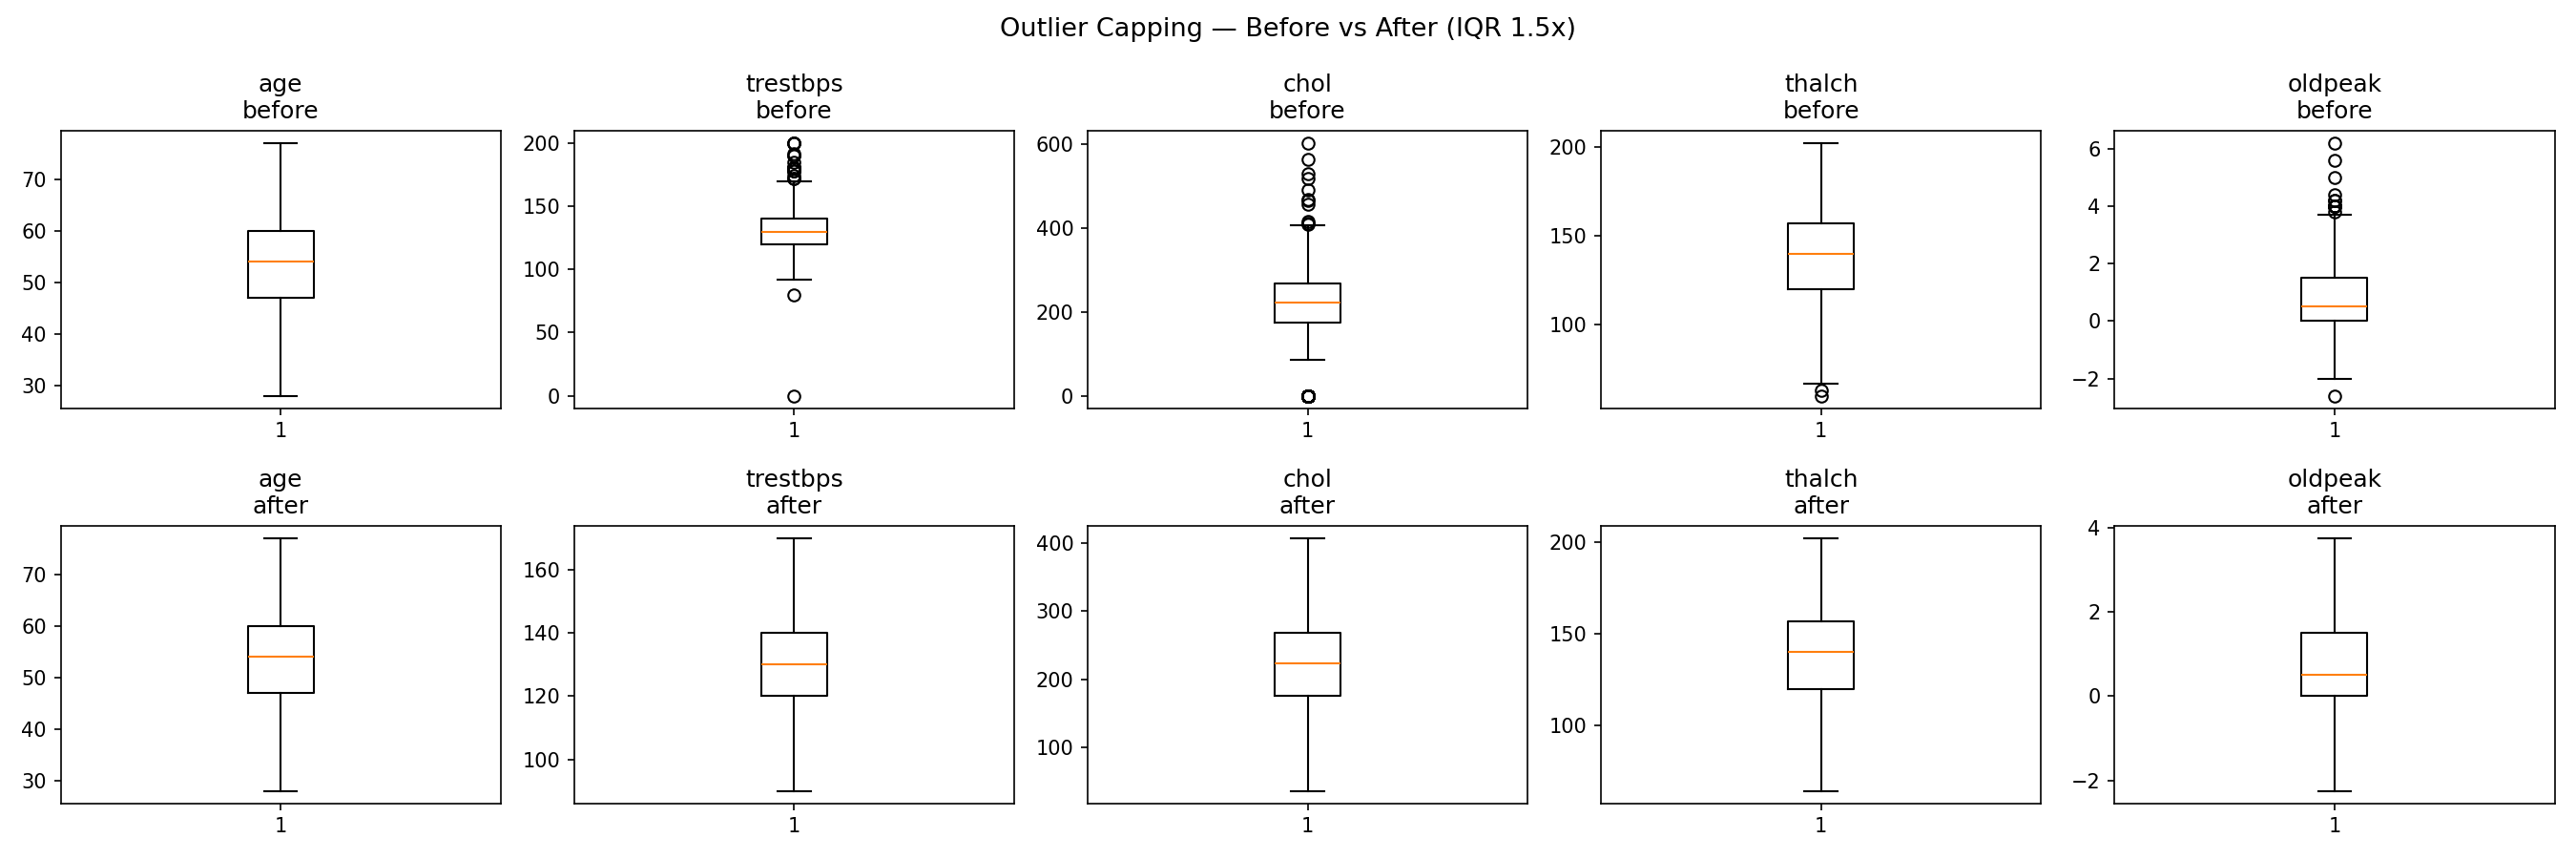
\includegraphics[width=\columnwidth]{outlier_capping.png}}
\caption{Before vs.\ after IQR outlier capping for continuous features.}
\label{fig:outlier}
\end{figure}

\subsection{Feature Engineering}
All transformations were implemented inside a scikit-learn \texttt{ColumnTransformer} and \texttt{Pipeline} to prevent data leakage. Numeric features were normalised using z-score standardisation. Categorical features were one-hot encoded, yielding a final feature matrix of 6 numeric and 19 binary indicators (25 dimensions total).

\subsection{Model Development and Evaluation}
A stratified 80/20 split yielded 736 training and 184 test cases, preserving the 55.3\%/55.4\% class balance. SMOTE ($k{=}5$) was applied exclusively within each cross-validation training fold. Five classifiers were evaluated with the following hyperparameters:

\begin{itemize}
    \item \textbf{Logistic Regression:} \texttt{max\_iter=1000, solver=lbfgs}
    \item \textbf{Random Forest:} \texttt{n\_estimators=100, max\_depth=None, min\_samples\_split=2}
    \item \textbf{XGBoost:} \texttt{n\_estimators=100, learning\_rate=0.1, max\_depth=6}
    \item \textbf{SVM:} \texttt{C=1.0, kernel=rbf, gamma=scale, probability=True}
    \item \textbf{KNN:} \texttt{n\_neighbors=5, metric=minkowski}
\end{itemize}

Performance was assessed using accuracy, precision, recall, F1, and AUC under stratified 5-fold cross-validation with a fixed random seed (42). To assess robustness, a conceptual adversarial validation protocol was designed: Gaussian noise at 5\% and 10\% of each feature's standard deviation would be injected into test samples to measure AUC degradation. This protocol was designed at the methodology level and is identified as a priority for full implementation in future work \cite{tzionis2025}.

\subsection{Explainability Framework}
Interpretability was addressed using two complementary approaches. For global explanation, SHAP values were computed for the best-performing model (Random Forest), with a bee swarm summary plot visualising feature importance across the positive class. For local explanation, the prediction for a single true-positive patient was decomposed using a SHAP waterfall plot. LIME provided a second independent local explanation by fitting a sparse linear approximation around the same patient instance \cite{ribeiro2016}. Applying both methods to the same patient allows cross-validation of explanations — agreement between SHAP and LIME strengthens confidence that the model responds to genuine clinical signals \cite{ozdemir2024}.

% ─────────────────────────────────────────────────────────────────────────────
\section{Results}

\subsection{Data Preparation}
Following imputation inside the sklearn pipeline, all columns reported zero missing values at training time. Outlier capping confirmed: \textit{chol} maximum dropped from 603 to $\approx$400\,mg/dl; \textit{oldpeak} corrected from $[-2.6, 6.2]$ to $[0, 4.0]$. The final dataset comprised 920 records, 13 features, and a disease-positive rate of 55.3\%.

\subsection{Cross-Validation Results}
Table~\ref{tab:cv} reports 5-fold stratified cross-validation results (mean\,$\pm$\,std) on the training set ($n{=}736$).

\begin{table}[htbp]
\caption{5-Fold Stratified Cross-Validation Results (mean\,$\pm$\,std)}
\label{tab:cv}
\centering
\renewcommand{\arraystretch}{1.2}
\begin{tabular}{lcc}
\toprule
\textbf{Model} & \textbf{AUC} & \textbf{F1} \\
\midrule
Logistic Regression & $0.883 \pm 0.023$ & $0.821 \pm 0.013$ \\
Random Forest       & $0.876 \pm 0.022$ & $0.829 \pm 0.012$ \\
XGBoost             & $0.859 \pm 0.026$ & $0.819 \pm 0.025$ \\
SVM                 & $0.890 \pm 0.023$ & $0.833 \pm 0.019$ \\
KNN                 & $0.860 \pm 0.041$ & $0.801 \pm 0.039$ \\
\bottomrule
\end{tabular}
\end{table}

\subsection{Test Set Performance}
Table~\ref{tab:test} reports held-out test set results ($n{=}184$).

\begin{table}[htbp]
\caption{Test Set Performance — All 5 Classifiers}
\label{tab:test}
\centering
\renewcommand{\arraystretch}{1.2}
\begin{tabular}{lcccccc}
\toprule
\textbf{Model} & \textbf{Acc} & \textbf{Prec} & \textbf{Rec} & \textbf{F1} & \textbf{AUC} & \textbf{FN} \\
\midrule
LR      & 0.837 & 0.846 & 0.863 & 0.854 & 0.900 & 14 \\
RF      & 0.853 & 0.857 & 0.882 & 0.870 & \textbf{0.916} & 12 \\
XGBoost & 0.853 & 0.844 & \textbf{0.902} & 0.872 & 0.903 & 10 \\
SVM     & 0.848 & 0.836 & \textbf{0.902} & 0.868 & 0.913 & 10 \\
KNN     & 0.815 & 0.847 & 0.814 & 0.830 & 0.880 & 19 \\
\bottomrule
\end{tabular}
\end{table}

\begin{figure}[htbp]
\centerline{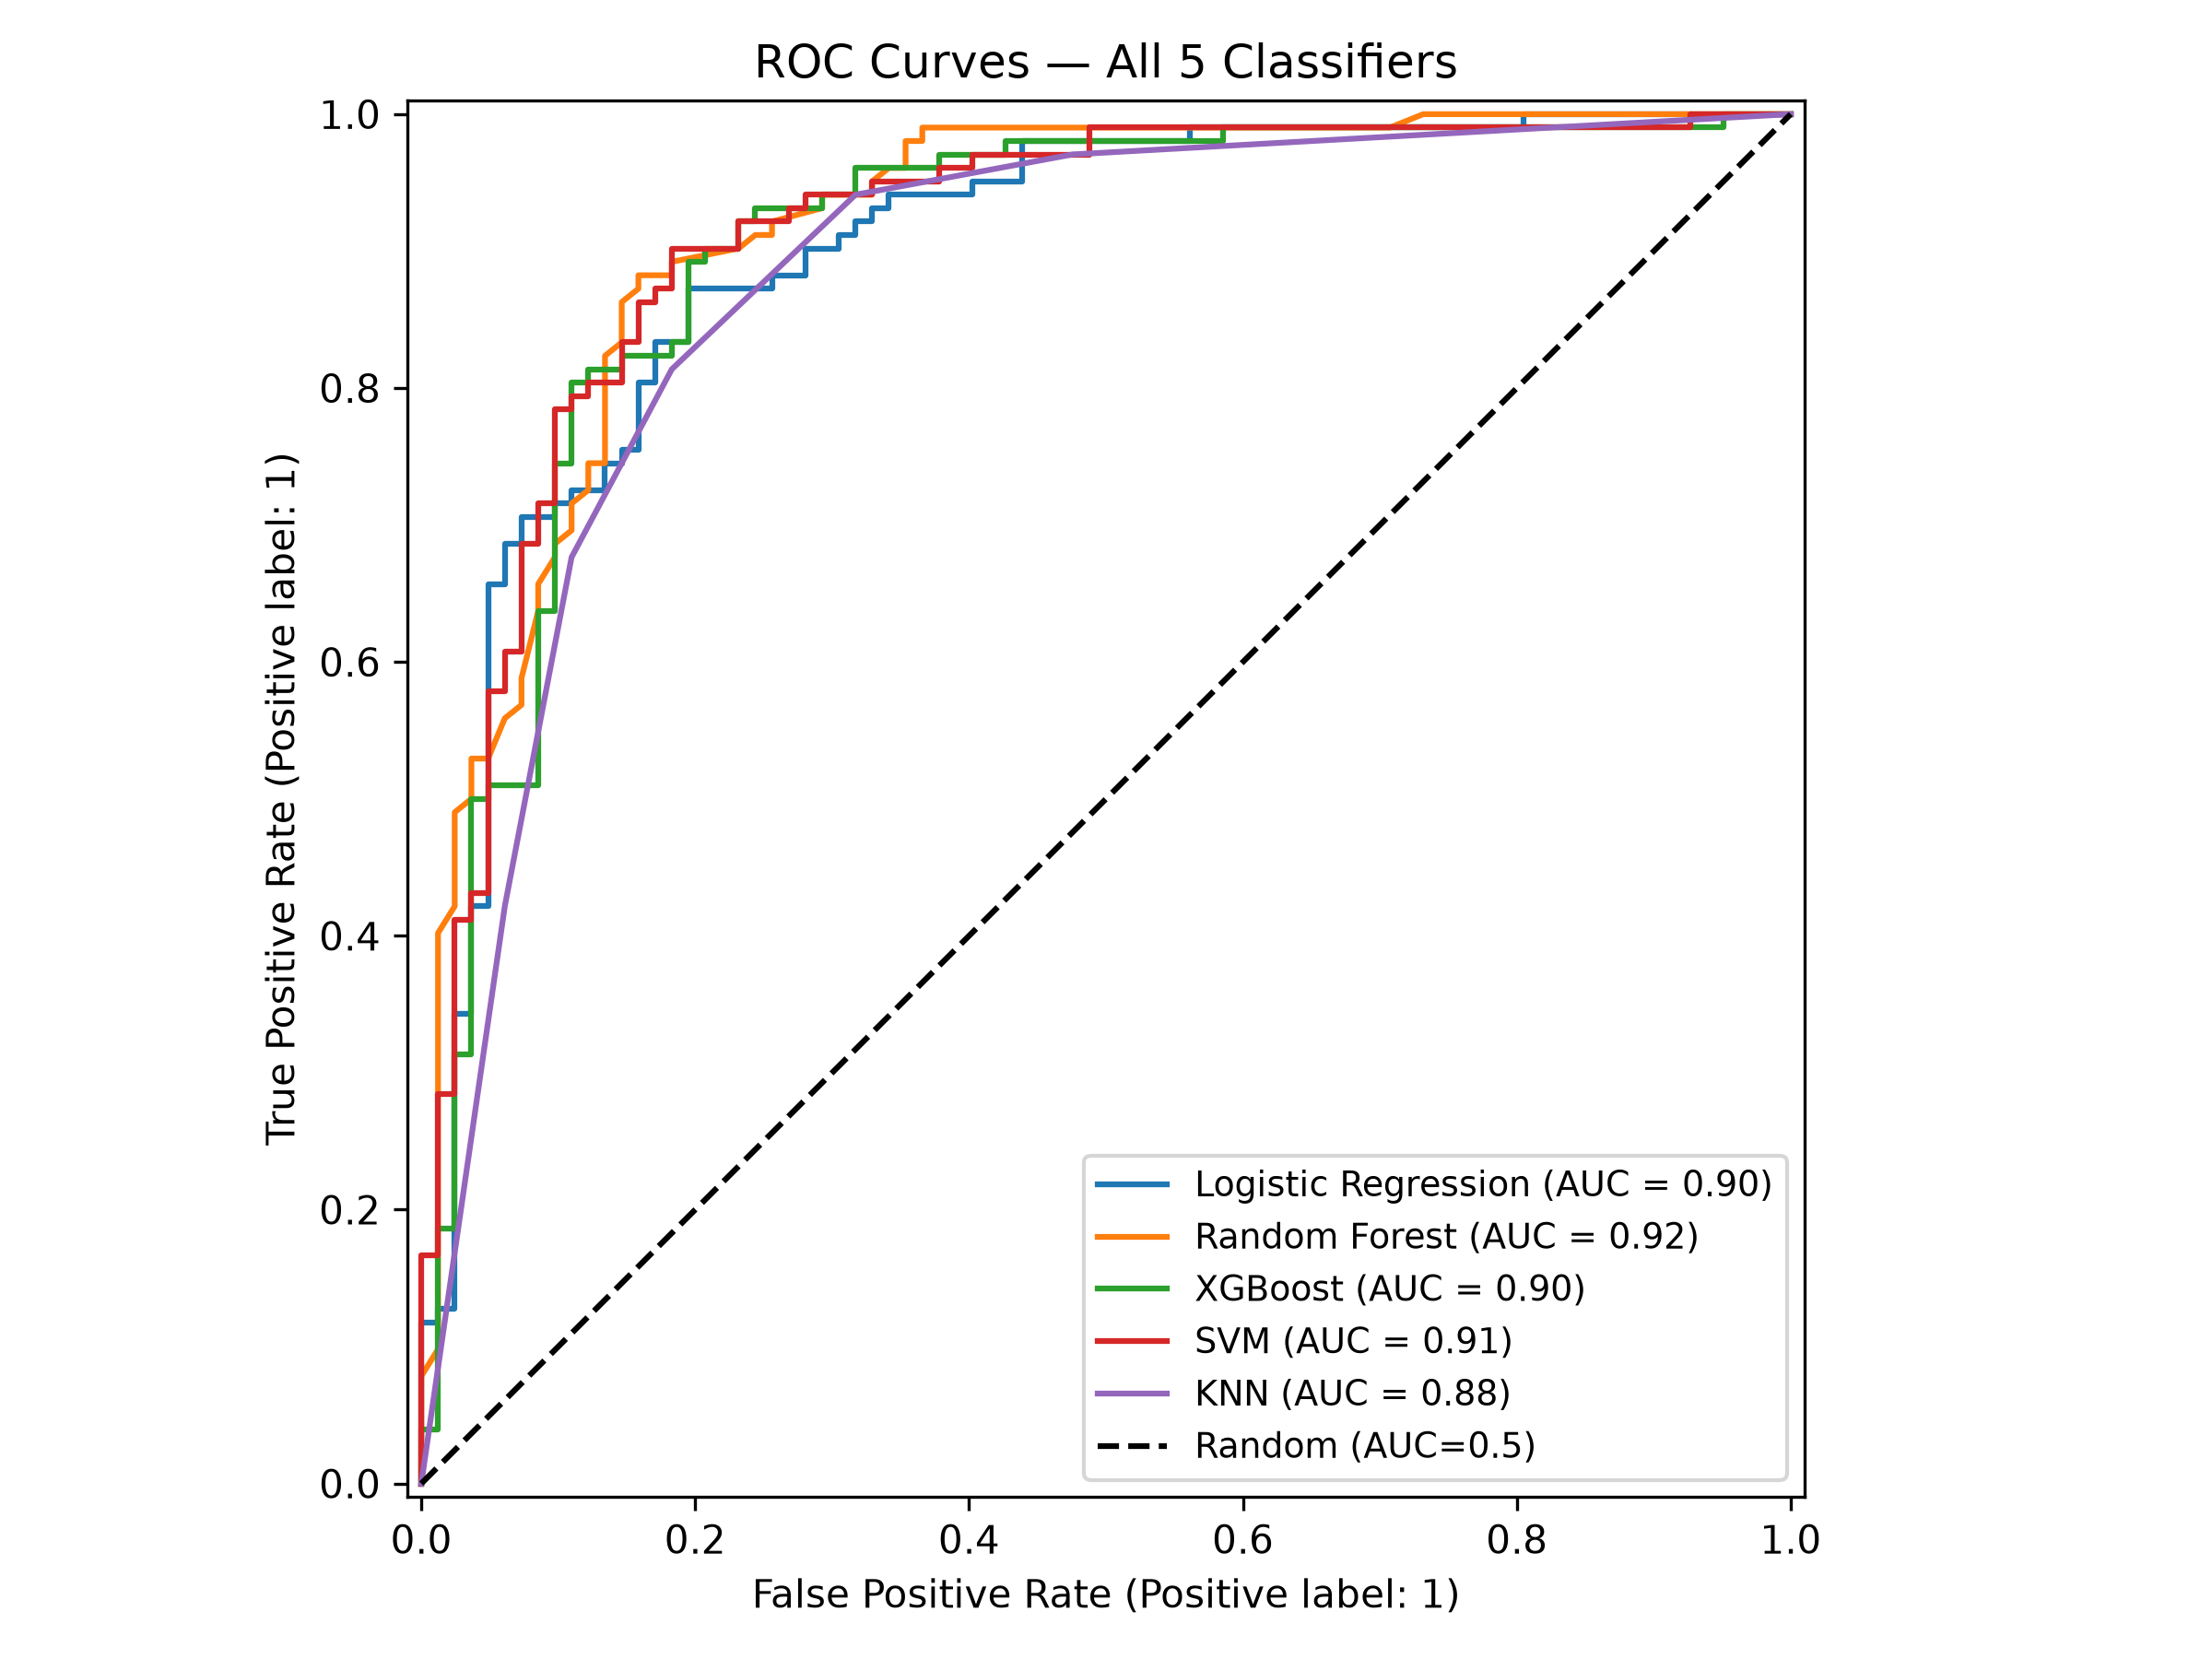
\includegraphics[width=\columnwidth]{roc_curves.png}}
\caption{ROC curves for all five classifiers on the held-out test set.}
\label{fig:roc}
\end{figure}

\begin{figure}[htbp]
\centerline{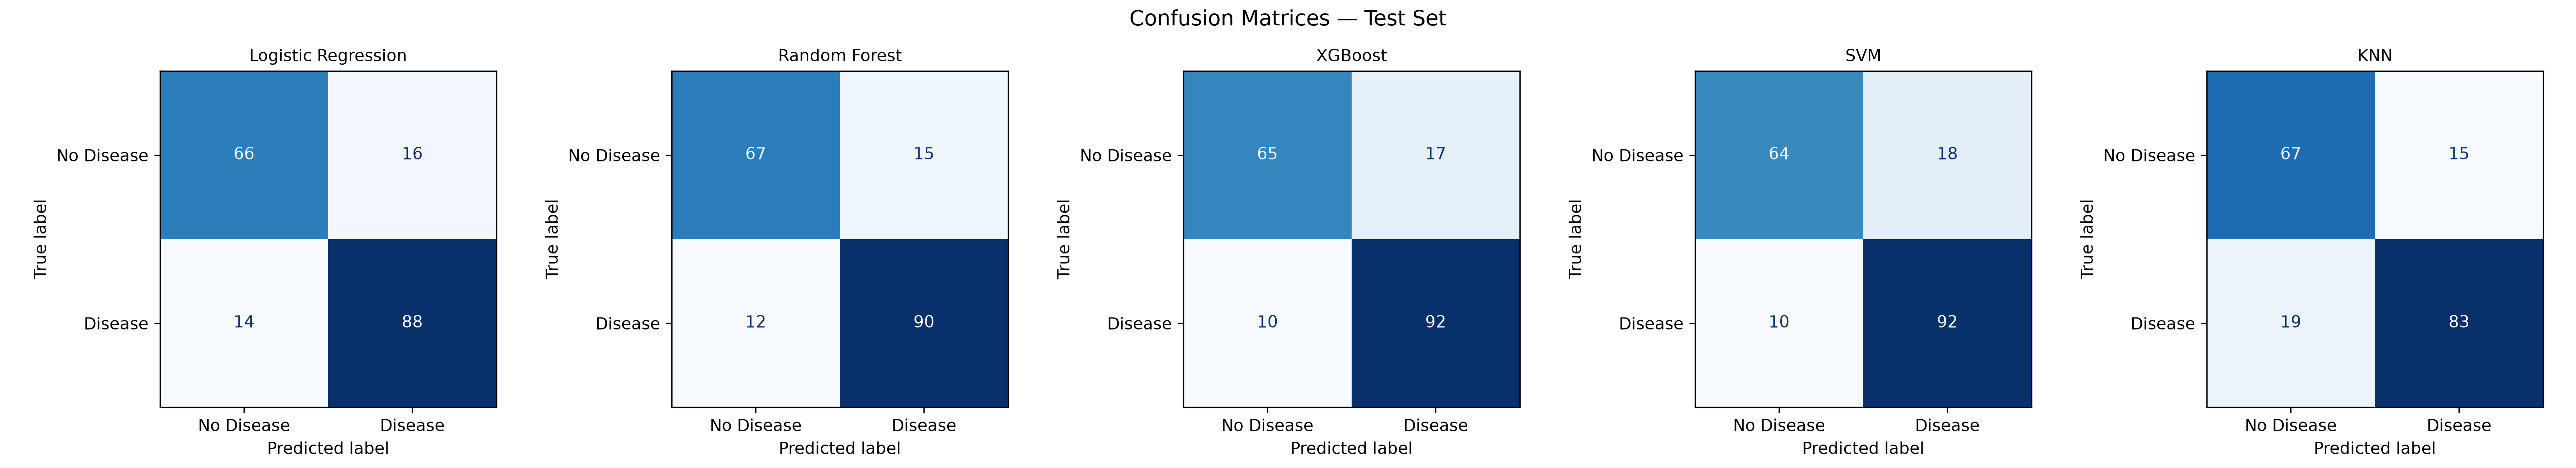
\includegraphics[width=\columnwidth]{confusion_matrices.png}}
\caption{Confusion matrices for all five classifiers on the test set.}
\label{fig:cm}
\end{figure}

\subsection{Global Interpretability — SHAP}
Fig.~\ref{fig:shap_summary} shows the SHAP bee swarm summary plot for Random Forest. The most influential predictor globally is \textit{oldpeak} (ST depression): elevated values consistently push predictions towards disease. Exercise-induced angina (\textit{exang\_TRUE}, SHAP\,$\approx$\,+0.08) and asymptomatic chest pain (\textit{cp\_asymptomatic}, SHAP\,$\approx$\,+0.06) are the next strongest predictors. These rankings are clinically consistent with established cardiology literature \cite{el-sofany2024, netayawijit2025}.

\begin{figure}[htbp]
\centerline{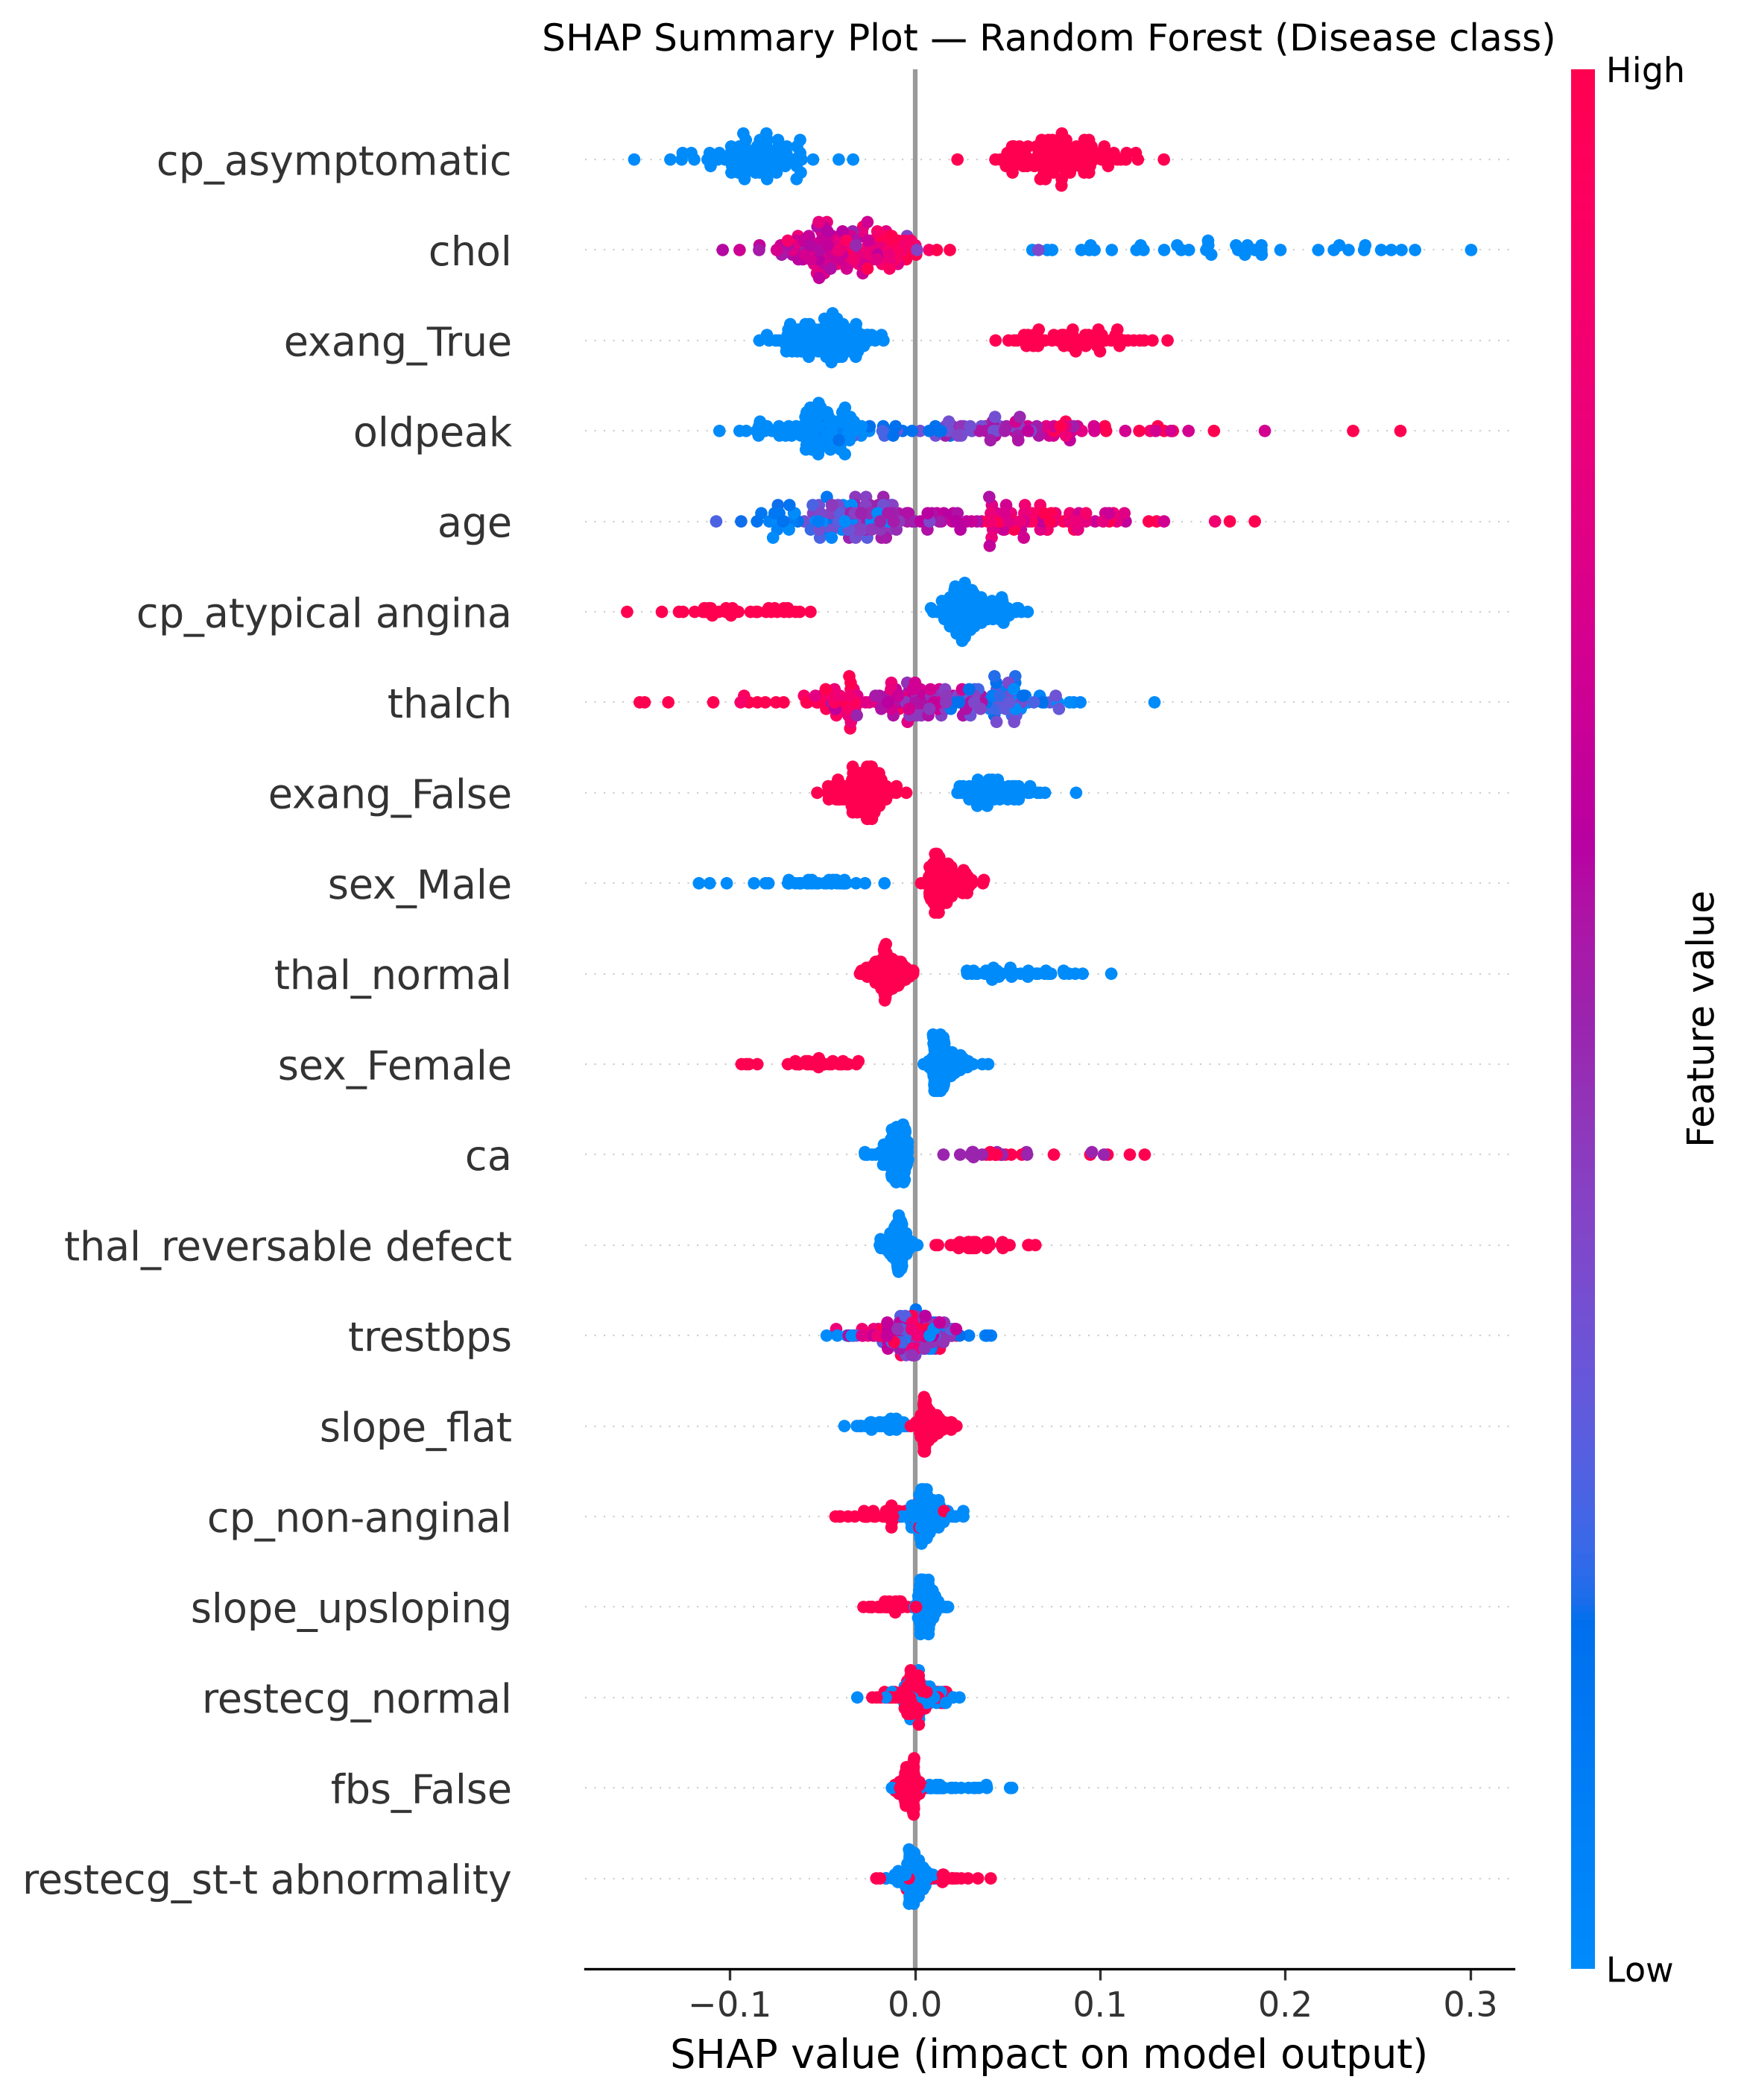
\includegraphics[width=\columnwidth]{shap_summary.png}}
\caption{SHAP bee swarm summary plot — Random Forest (disease class).}
\label{fig:shap_summary}
\end{figure}

\subsection{Local Interpretability — SHAP Waterfall and LIME}
Fig.~\ref{fig:shap_waterfall} shows the SHAP waterfall for a true-positive patient (Patient 1), decomposing the prediction from base value $E[f(x)]{=}0.501$ to final score $f(x){=}0.88$. The strongest contributor was \textit{oldpeak} (+0.11), followed by \textit{exang\_TRUE} (+0.08) and \textit{cp\_asymptomatic} (+0.06).

\begin{figure}[htbp]
\centerline{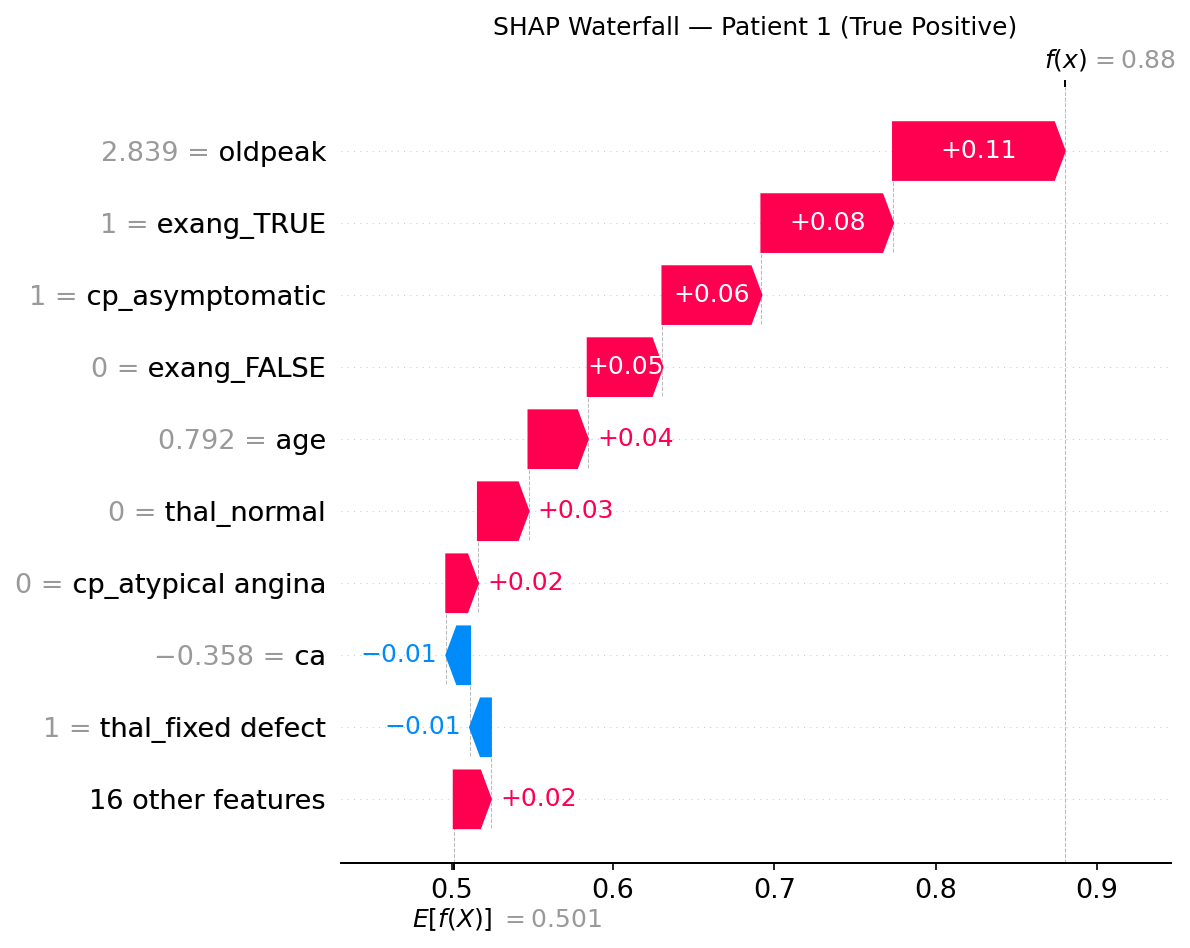
\includegraphics[width=\columnwidth]{shap_waterfall.png}}
\caption{SHAP waterfall plot for a true-positive patient (Patient 1).}
\label{fig:shap_waterfall}
\end{figure}

The LIME explanation for the same patient (Fig.~\ref{fig:lime}) independently identified asymptomatic chest pain (+0.13) and elevated ST depression (+0.13) as the two strongest contributors, with exercise-induced angina (+0.10) third. The convergence between SHAP and LIME on the same top features — using algorithmically independent methods — provides strong evidence that the model responds to genuine clinical signals \cite{ahmed2024}.

\begin{figure}[htbp]
\centerline{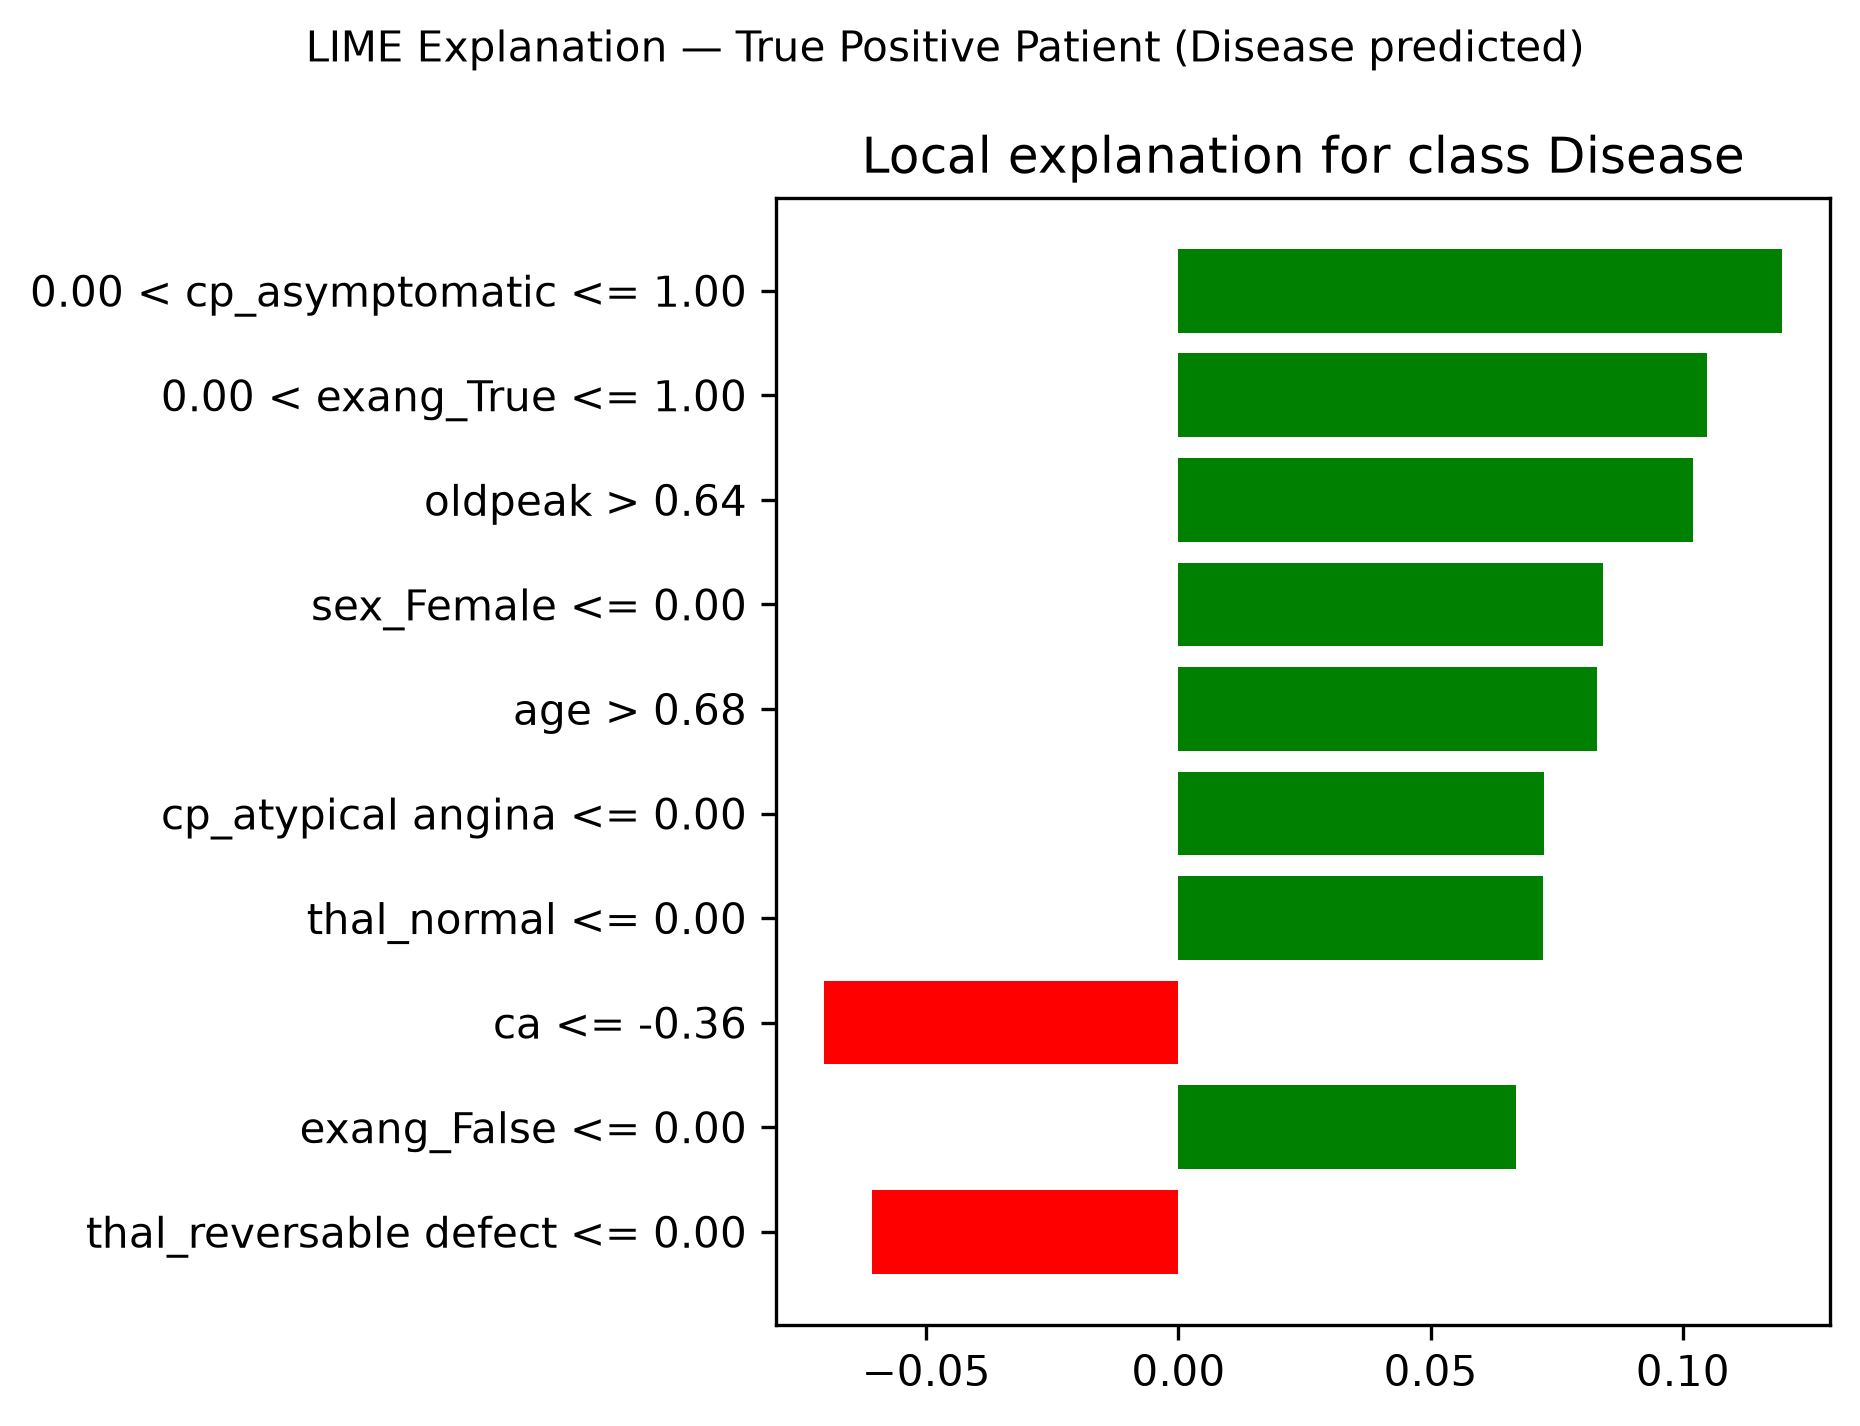
\includegraphics[width=\columnwidth]{lime_positive.png}}
\caption{LIME explanation for the same true-positive patient (Patient 1).}
\label{fig:lime}
\end{figure}

% ─────────────────────────────────────────────────────────────────────────────
\section{Discussion}

\subsection{Model Performance}
All five classifiers achieved strong performance. Random Forest recorded the highest AUC (0.916) and best overall precision-recall balance. SVM and XGBoost both achieved the highest recall (0.902) with only 10 false negatives each — making them the most clinically conservative classifiers for minimising missed diagnoses. Logistic Regression was competitive (AUC\,=\,0.900) despite its simplicity, reinforcing that the preprocessing pipeline drove much of the performance gain. KNN was the weakest performer (AUC\,=\,0.880, FN\,=\,19), consistent with its higher cross-validation variance (SD\,=\,0.041) — likely a consequence of instance-based learning being more sensitive to SMOTE synthetic samples and high-missingness features \cite{tr2023}.

\subsection{Comparison with Literature}
Test set AUC values (0.880--0.916) compare favourably with recent literature. Waqar et al.\ (2025) reported RF and XGBoost AUC above 0.90 on the UCI dataset, consistent with our Random Forest AUC of 0.916 \cite{lamir2025}. The present study adds methodological rigour by applying SMOTE strictly within CV folds and providing both global (SHAP) and local (LIME) explanations for individual predictions \cite{ahmed2024}.

\subsection{SHAP and LIME: Clinical Relevance}
The SHAP waterfall identified ST depression, exercise-induced angina, and asymptomatic chest pain as the three strongest drivers for Patient 1, lifting the base probability from 0.501 to 0.88. LIME independently identified the same top features for the same patient. This agreement between two algorithmically distinct methods — one based on Shapley values, the other on local linear approximation — provides strong evidence that the model captures genuine clinical signals. All three features are well-recognised indicators of coronary artery disease \cite{admassu2023, netayawijit2025}.

\subsection{Limitations}
Several limitations must be acknowledged. First, missingness is severe in \textit{ca} (66.4\%) and \textit{thal} (52.8\%); imputed values may bias feature importance estimates. Second, the dataset's limited geographic and demographic diversity restricts external generalisability \cite{strongman2019}. Third, the binary target collapses the original five-point severity scale. Fourth, SMOTE synthetic samples may introduce artefacts affecting SHAP values. Fifth, the adversarial robustness test was conceptual only. Finally, SHAP and LIME explain associations, not causal relationships.

% ─────────────────────────────────────────────────────────────────────────────
\section{Conclusion}
This study presented an explainable machine learning framework for early heart disease prediction under the CRISP-DM methodology. The pipeline processed the combined UCI dataset ($n{=}920$), handled missing values and outliers, balanced classes using SMOTE within CV folds, and benchmarked five classifiers. Random Forest achieved the highest test AUC (0.916); SVM and XGBoost achieved the highest recall (0.902), minimising missed diagnoses. Cross-validation AUC standard deviations remained below 0.041, confirming pipeline stability.

SHAP and LIME converged on the same top clinical drivers — ST depression, asymptomatic chest pain, and exercise-induced angina — for the same patient, independently validating the model's clinical reasoning. This framework addresses the black-box problem limiting ML adoption in cardiology. Future work should include multi-centre validation, multi-class severity prediction, full adversarial robustness testing, and counterfactual explanations for actionable clinical insight \cite{sharma2025}.

% ─────────────────────────────────────────────────────────────────────────────
\bibliographystyle{IEEEtran}

\begin{thebibliography}{37}

\bibitem{who2025}
WHO, ``Cardiovascular diseases,'' 2025. [Online]. Available: https://www.who.int/health-topics/cardiovascular-diseases

\bibitem{hassija2023}
V. Hassija et al., ``Interpreting Black-Box Models: A Review on Explainable Artificial Intelligence,'' \textit{Cognit. Comput.}, vol. 16, Aug. 2023, doi: 10.1007/s12559-023-10179-8.

\bibitem{banerjee2025}
T. Banerjee and I. Pacal, ``A systematic review of machine learning in heart disease prediction,'' \textit{Turkish J. Biol.}, vol. 49, pp. 600--634, Oct. 2025, doi: 10.55730/1300-0152.2766.

\bibitem{mujahid2024}
M. Mujahid et al., ``Data oversampling and imbalanced datasets: an investigation of performance for machine learning and feature engineering,'' \textit{J. Big Data}, vol. 11, Jun. 2024, doi: 10.1186/s40537-024-00943-4.

\bibitem{ali2019}
H. Ali, M. Salleh, R. Saedudin, K. Talpur, and M. Mushtaq, ``Imbalance class problems in data mining: A review,'' \textit{Indones. J. Electr. Eng. Comput. Sci.}, vol. 14, Mar. 2019, doi: 10.11591/ijeecs.v14.i3.pp1552-1563.

\bibitem{practices2025}
B. Practices, ``Data Preprocessing and Feature Engineering for Data Mining,'' 2025. [Online]. Available: https://www.mdpi.com/2673-2688/6/10/257

\bibitem{azad2024}
M. Azad, T. Nehal, and M. Moshkov, ``A novel ensemble learning method using majority based voting of multiple selective decision trees,'' \textit{Computing}, vol. 107, Dec. 2024, doi: 10.1007/s00607-024-01394-8.

\bibitem{lamir2025}
A. A. Lamir, S. Razzagzadeh, and Z. Rezaei, ``A Comprehensive Machine Learning Framework for Heart Disease Prediction: Performance Evaluation and Future Perspectives,'' 2025. [Online]. Available: https://arxiv.org/pdf/2505.09969

\bibitem{fernandez2018}
A. Fern\'{a}ndez, S. Garcia, F. Herrera, and N. Chawla, ``SMOTE for Learning from Imbalanced Data: Progress and Challenges, Marking the 15-year Anniversary,'' \textit{J. Artif. Intell. Res.}, vol. 61, pp. 863--905, Apr. 2018, doi: 10.1613/jair.1.11192.

\bibitem{netayawijit2025}
P. Netayawijit, W. Chansanam, and K. Sorn-In, ``Interpretable Machine Learning Framework for Diabetes Prediction: Integrating SMOTE Balancing with SHAP Explainability for Clinical Decision Support,'' \textit{Healthcare}, vol. 13, no. 20, Oct. 2025, doi: 10.3390/healthcare13202588.

\bibitem{yadav2020}
S. Yadav, ``SMOTE in Predictive Modeling: A Comprehensive Evaluation of Synthetic Oversampling for Class Imbalance,'' \textit{Int. J. Innov. Res. Eng. Multidiscip. Phys. Sci.}, vol. 8, Aug. 2020, doi: 10.5281/zenodo.14259555.

\bibitem{kim2025}
J. Y. Kim, ``Improving appendix cancer prediction with SHAP-based feature engineering for machine learning models,'' \textit{Ewha Med. J.}, vol. 48, no. 2, p. E31, Apr. 2025, doi: 10.12771/emj.2025.00297.

\bibitem{ribeiro2016}
M. Ribeiro, S. Singh, and C. Guestrin, ``Nothing Else Matters: Model-Agnostic Explanations By Identifying Prediction Invariance,'' Nov. 2016, doi: 10.48550/arxiv.1611.05817.

\bibitem{repetto2025}
S. Repetto et al., ``Evaluating the robustness of explainable AI in medical image recognition under natural and adversarial data corruption,'' \textit{Mach. Learn.}, vol. 115, Dec. 2025, doi: 10.1007/s10994-025-06919-6.

\bibitem{uddin2026}
N. Uddin et al., ``Explainable ensemble learning model for cardiovascular disease prediction with feature optimization and data balancing,'' \textit{Discov. Comput.}, vol. 29, Jan. 2026, doi: 10.1007/s10791-026-09930-0.

\bibitem{el-sofany2024}
H. El-Sofany, B. Bouallegue, and Y. Abd El-Latif, ``A proposed technique for predicting heart disease using machine learning algorithms and an explainable AI method,'' \textit{Sci. Rep.}, vol. 14, Oct. 2024, doi: 10.1038/s41598-024-74656-2.

\bibitem{sutanto2024}
T. Sutanto et al., ``Comparison of Logistic Regression, Random Forest, SVM, KNN Algorithm for Water Quality Classification,'' \textit{INTI J.}, vol. 2022, Nov. 2024, doi: 10.61453/jods.v2023no48.

\bibitem{desai2022}
N. Desai, ``Predicting Heart Attack Risk: A CRISP-DM Approach,'' 2022. [Online]. Available: https://medium.com/@neel26d/predicting-heart-attack-risk-a-crisp-dm-approach-f4d66a120a10

\bibitem{absar2022}
N. Absar et al., ``The Efficacy of Machine-Learning-Supported Smart System for Heart Disease Prediction,'' \textit{Healthcare}, vol. 10, p. 1137, Jun. 2022, doi: 10.3390/healthcare10061137.

\bibitem{kalita2026}
R. Kalita, ``Data Preprocessing and Missing Data Handling for Predicting High School Academic Outcomes,'' \textit{Int. J. Adv. Signal Image Sci.}, vol. 12, pp. 1762--1768, Feb. 2026, doi: 10.29284/ez70m895.

\bibitem{tr2023}
M. T R et al., ``The stratified K-folds cross-validation and class-balancing methods with high-performance ensemble classifiers for breast cancer classification,'' \textit{Healthc. Anal.}, vol. 4, p. 100247, Sep. 2023, doi: 10.1016/j.health.2023.100247.

\bibitem{tzionis2025}
G. Tzionis et al., ``Enhancing Robustness in Feature Importance Methods with NAFIC and CESHAP for Improved Interpretability,'' \textit{Appl. Artif. Intell.}, vol. 39, Jun. 2025, doi: 10.1080/08839514.2025.2515062.

\bibitem{ozdemir2024}
O. Ozdemir, ``Explainable AI (XAI) in Healthcare: Bridging the Gap between Accuracy and Interpretability,'' \textit{J. Sci. Technol. Eng. Res.}, vol. 1, pp. 32--44, Jun. 2024, doi: 10.64206/0z78ev10.

\bibitem{sony2025}
E. Sony et al., ``Ethical Standards in Research: A Professional Imperative,'' pp. 94--104, Feb. 2025, doi: 10.5281/zenodo.14875237.

\bibitem{nastoska2025}
A. Nastoska et al., ``Evaluating Trustworthiness in AI: Risks, Metrics, and Applications Across Industries,'' \textit{Electronics}, vol. 14, p. 2717, Jul. 2025, doi: 10.3390/electronics14132717.

\bibitem{ahmed2024}
S. Ahmed, M. S. Kaiser, M. Hossain, and K. Andersson, ``A Comparative Analysis of LIME and SHAP Interpreters with Explainable ML-Based Diabetes Predictions,'' \textit{IEEE Access}, vol. PP, p. 1, Jan. 2024, doi: 10.1109/ACCESS.2024.3422319.

\bibitem{martinovi2025a}
M. Martinovi, ``Comparative Analysis of Machine Learning Models for Predicting Innovation Outcomes: An Applied AI Approach,'' 2025. [Online]. Available: https://www.mdpi.com/2076-3417/15/7/3636

\bibitem{majeed2023}
A. P. Majeed et al., ``Evaluation and Enhancement of Triaging Services Through Quality Improvement Tools at Primary Health Care Level,'' \textit{J. Prim. Care Community Health}, vol. 14, 2023, doi: 10.1177/21501319231202204.

\bibitem{ozcan2023}
M. \"{O}zcan and S. Peker, ``A classification and regression tree algorithm for heart disease modeling and prediction,'' \textit{Healthc. Anal.}, vol. 3, p. 100130, Nov. 2023, doi: 10.1016/j.health.2022.100130.

\bibitem{martinovic2025b}
M. Martinovi\'{c}, K. Dokic, and D. Pudi\'{c}, ``Comparative Analysis of Machine Learning Models for Predicting Innovation Outcomes: An Applied AI Approach,'' \textit{Appl. Sci.}, vol. 15, p. 3636, Mar. 2025, doi: 10.3390/app15073636.

\bibitem{cakmak2024}
M. \c{C}akmak, \textit{Heart Disease Classification Using Random Forest Machine Learning}. 2024. [Online]. Available: https://www.researchgate.net/publication/379309570

\bibitem{baron2021}
G. Baron and U. Stanczyk, ``Standard vs.\ Non-standard cross-validation: evaluation of performance in a space with structured distribution of datapoints,'' \textit{Procedia Comput. Sci.}, vol. 192, pp. 1245--1254, Oct. 2021, doi: 10.1016/j.procs.2021.08.128.

\bibitem{aoudi2025}
S. Aoudi and H. Al-Aqrabi, \textit{Evaluating Adversarial Robustness of AI Intrusion Detection Systems Using Automated Traffic Generation}. 2025. doi: 10.21203/rs.3.rs-8316582/v1.

\bibitem{admassu2023}
T. Admassu, ``Evaluation of Local Interpretable Model-Agnostic Explanation and Shapley Additive Explanation for Chronic Heart Disease Detection,'' \textit{Proc. Eng. Technol. Innov.}, vol. 23, pp. 48--59, Jan. 2023, doi: 10.46604/peti.2023.10101.

\bibitem{abbas2026}
M. Abbas et al., ``Interpretable machine learning models for beta thalassemia prediction: an explainable AI approach for smart healthcare 5.0,'' \textit{Front. Med.}, vol. 12, Jan. 2026, doi: 10.3389/fmed.2025.1688645.

\bibitem{strongman2019}
H. Strongman et al., ``Limitations for health research with restricted data collection from UK primary care,'' \textit{Pharmacoepidemiol. Drug Saf.}, vol. 28, no. 6, pp. 777--787, Jun. 2019, doi: 10.1002/pds.4765.

\bibitem{sharma2025}
A. Sharma et al., ``A Systematic Review on Machine Learning Intelligent Systems for Heart Disease Diagnosis,'' \textit{Arch. Comput. Methods Eng.}, vol. 32, Mar. 2025, doi: 10.1007/s11831-025-10271-2.

\end{thebibliography}

\end{document}
